\newpage
\section{Introduction}
\paragraph{}
Ce projet a été réalisé par quatre étudiants de première année de
Master Informatique de l'Université de Bordeaux (parcours Génie
Logiciel), dans le cadre de l'UE Projet de Programmation.

\subsection{Un outil pour assister l'improvisation musicale}
\paragraph{}
Le projet a été proposé par Myriam Desainte-Catherine, chercheur au
Studio de Création et de Recherche en Informatique et Musiques
Expérimentales (SCRIME) et enseignante à l'ENSEIRB-MATMECA, et Yacine
Amarouchene, physicien du Laboratoire d'Onde et Matière d'Aquitaine
(LOMA). Il a été pensé comme un outil d'aide à "l'improvisation
musicale", un dispositif permettant d'aider un groupe de musiciens à
improviser mais permettant aussi de mieux comprendre la nature de
l'improvisation en musique.

\begin{figure}[H]
      \centering
      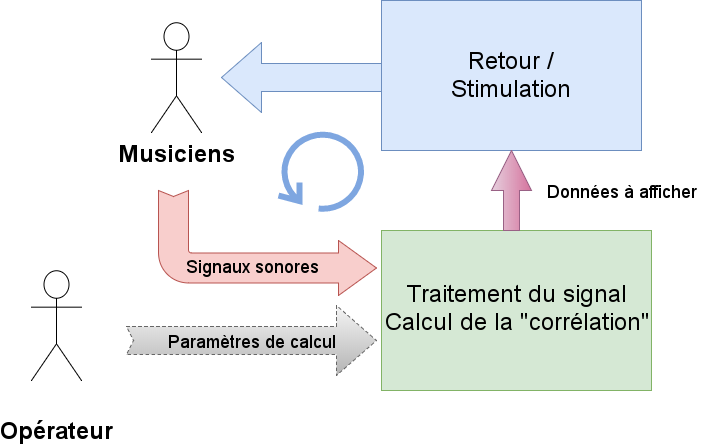
\includegraphics[scale=0.5]{assets/principe_global.png}
      \caption{Principe général du projet}
      \label{principe général}
\end{figure}
\paragraph{}
Le schéma ci-dessus résume le principe général du projet. Les
musiciens jouent librement, et leur musique une fois transformée en
signal discret, pourra alors être traitée pour que se dégage en sortie
un résultat que l'on appelle la "corrélation" (voir la section
suivante). Ensuite, il s'agit d'établir un retour (visuel, audio) pour
que les musiciens puissent être stimulés. L'objectif de cet outil est
de reproduire la boucle décrite sur le schéma.

\subsection{Improvisation et corrélation}
\paragraph{}

Il est essentiel de comprendre ces deux notions afin de bien situer
l'intérêt du projet.

\paragraph{}
Lors d'une improvisation en groupe, des musiciens jouent sans règle
établie ; ils cherchent alors à fournir à leur auditoire une
production cohérente, ou du moins au sein de laquelle chaque musicien
joue un rôle dans l'harmonie du morceau en s'accordant avec ses
pairs. La relation qui unit le jeu de deux musiciens et évalue la
qualité de leur accord porte un nom : c'est la corrélation.
\paragraph{}
Au sens premier et basique du terme, la corrélation est le rapport
réciproque entre deux éléments. En statistiques, on parle souvent de
corrélation pour mesurer l'intensité de la liaison existant entre deux
variables.
\paragraph{}
En musique, il n'existe pas une mais un nombre indéfini de "fonctions
de corrélation" potentiellement existantes, dont la complexité et les
paramètres varient. Pour établir ce "rapport réciproque" entre deux
signaux sonores, on pourrait comparer leurs tempos, leurs amplitudes,
leurs volumes sonores... "Comprendre" la corrélation et
l'improvisation, dans le cadre de ce projet, c'est aussi trouver,
inventer la fonction de corrélation qui répond le mieux aux besoins
d'un groupe d'improvisateurs. Une bonne fonction de corrélation, dans
ce cadre spécifique, est une fonction qui fait en sorte qu'un groupe
de musiciens joue un morceau plus satisfaisant lorsque ses membres
sont davantage corrélés ("découvrir" la fonction de corrélation relève
ici du rôle de l'utilisateur ou du physicien, le logiciel que nous
implémentons n'étant qu'un assistant dans cette démarche).
\paragraph{}
Les traductions graphiques de signaux sonores par transformée de
Fourier peuvent jouer le rôle des courbes dont on mesure la
corrélation. Tout au long du déroulement de notre projet, nous
travaillons uniquement sur des fonctions de corrélation portant sur la
comparaison des signaux graphiques obtenus à partir des pistes
sonores.

%Dans le cadre de l'étude de signaux sonores, nous faisons le calcul de
%corrélation entre deux signaux. Cette corrélation cherche à mesurer
%la similarité entre ces deux signaux suivant
%différents critères, par exemple la longueur d'onde.

\subsection{L'existant}
\paragraph{}
Ce projet a été initié par les clients précédemment cités il y a plus
d'un an. Nous sommes le troisième groupe à travailler sur ce projet et
développons donc sur la base des travaux réalisés successivement par
nos prédécesseurs.

\subsubsection{Premiers travaux réalisés sur le projet}
\paragraph{}
Les premiers travaux portant sur ce projet ont été réalisés par un
groupe de six étudiants de l'ENSEIRB-MATMECA. Cette équipe est la
première à réaliser un programme informatique analysant et comparant
des pistes mono-instrumentales pour évaluer leurs corrélations. Ce
programme, prenant en entrées des pistes sonores, retourne une matrice
graphique prenant les mêmes pistes en abscisses et en ordonnées et
retournant pour chaque case une couleur permettant d'évaluer la
corrélation existant entre les deux pistes correspondantes grâce à un
code couleur précis.

\begin{figure}[H]
 \centering
 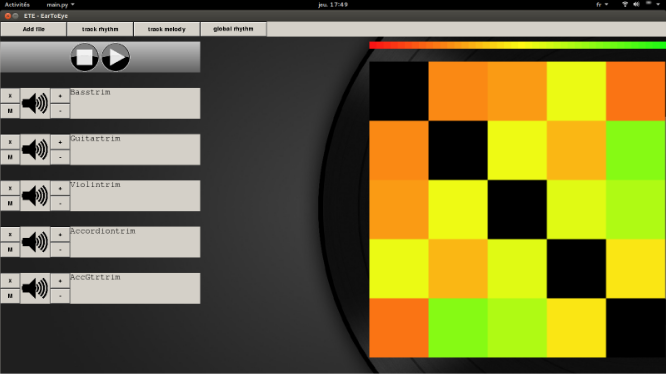
\includegraphics[scale=0.5]{assets/matriceenseirb.png}
 \caption{Capture d'écran du projet mené par les étudiants de l'ENSEIRB}
 \label{matrice-enseirb}
\end{figure}

\paragraph{}
Ci-dessus, la matrice obtenue à l'issue d'un test du programme. Plus
la couleur d'une case est proche du vert, plus la corrélation entre
les deux pistes correspondant au point d'abscisse et au point
d'ordonnée est élevée. À l'inverse, une case dont la couleur est
proche du rouge indique que les deux pistes évaluées sont
décorrélées. La corrélation d'une piste mono-instrumentale avec
elle-même, qui donne toujours un résultat maximal, n'est pas calculée,
ce qui se traduit sur le résultat graphique ci-dessus par une
diagonale de cases noires. La matrice de corrélation est donc
systématiquement symétrique.

\subsubsection{Le système embarqué BELA}
\paragraph{}
Avant de confier la suite du projet à d'autres étudiants, nos clients
ont choisi de changer de support et ont opté pour l'utilisation d'un
système embarqué particulier : BELA.\cite{BELA}

\paragraph{}
Ce choix s'explique par la mobilité du support, mais également par le
fait que BELA est basé sur un système appelé Xenomai Linux, un
framework qui ajoute au noyau Linux des éléments permettant de traiter
des opérations en temps réel.\cite{XENOMAI} Cela permet au système de
faire du traitement audio en temps réel avec un temps de latence
extrêmement faible (100 microsecondes).

\begin{figure}[H]
 \centering
 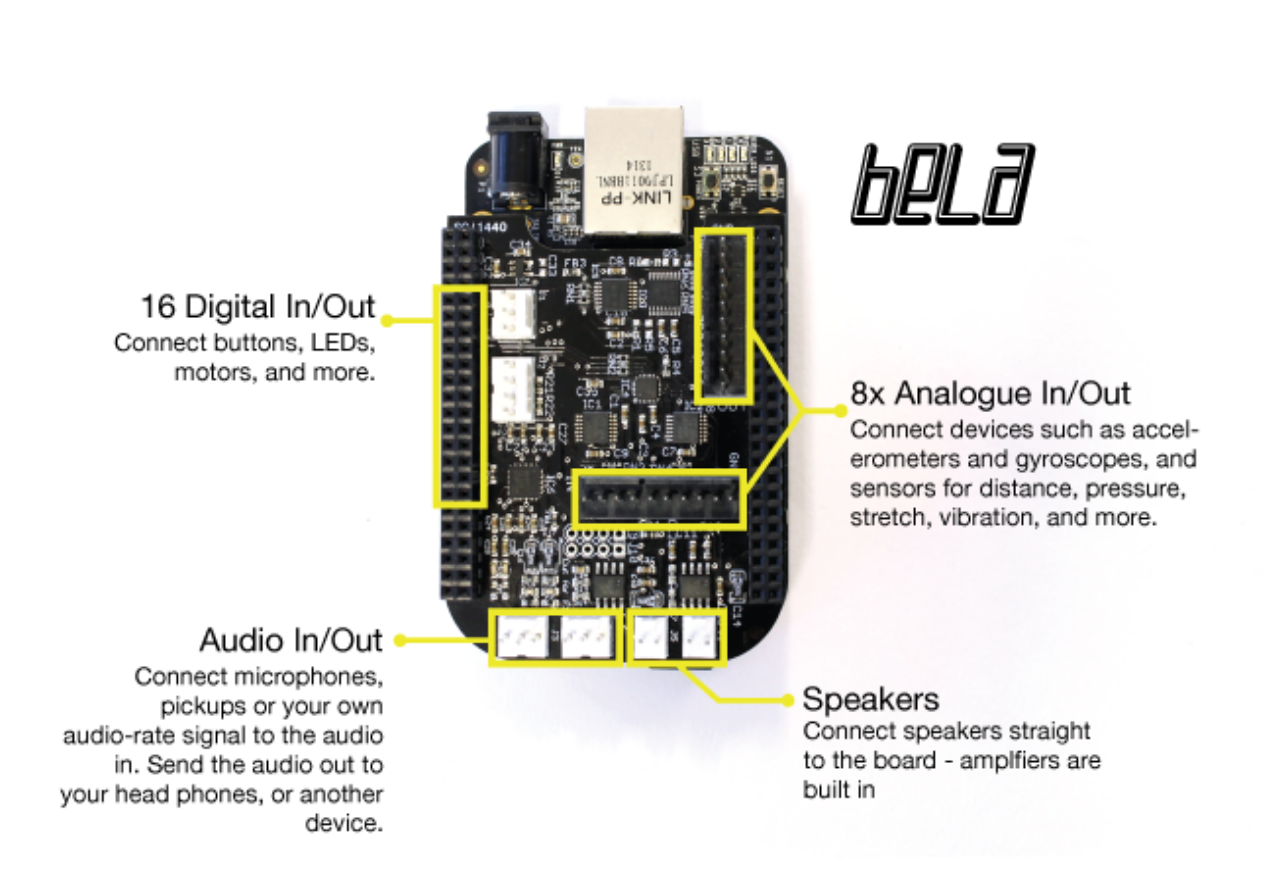
\includegraphics[scale=0.2]{assets/bela.png}
 \caption{Capture de la documentation proposée par le site officiel de Bela}
 \label{bela}
\end{figure}

\paragraph{}
L'aperçu du dispositif externe de BELA présenté ci-après témoigne
notamment de la présence d'entrées analogiques pour connecter des
instruments électriques ou enregistreurs sonores. On comprend alors
que le rôle de BELA au sein de ce projet est l'utilisation d'un
programme en temps réel par un groupe d'improvisateurs,
similaire à celui implémenté par les étudiants de l'ENSEIRB, dont les
instruments seraient connectés à cet outil. Ce dernier dispose déjà de
fonctions de traitement du son codées en C++, mais revêt surtout un intérêt
pour les développeurs, qui peuvent librement modifier et enrichir son
programme.
\paragraph{}
Le dispositif externe BELA comprend huit entrées analogiques et deux
entrées audio. Son architecture lui permet d'interpréter parallèlement
jusqu'à seize fichiers audio numériques supplémentaires.
\paragraph{}
Le framework de BELA permet l'implémentation de programmes divers par
son utilisateur à partir de deux fichiers sources codés en C++ : le
"main" exécutant le programme principal et le "render" qui met à jour
l'analyse des signaux reçus en entrée.

\subsubsection{Un logiciel d'aide à l'improvisation musicale}
\paragraph{}
En juin 2017, Jérémy Lixandre, membre des six étudiants ayant amorcé
le projet, poursuit seul ces travaux en s'aidant cette fois de BELA,
au cours d'un stage de deux mois au laboratoire du SCRIME de
Bordeaux. Il reprend le concept de "matrice de corrélation" mais
doit reprendre l'implémentation du logiciel à zéro, puisqu'il
abandonne le langage Python utilisé lors des premiers travaux pour
passer à la programmation C++ exigée par le code de BELA.
\paragraph{}
De plus, il relègue les travaux de recherche sur la corrélation et ses
formules, des tâches relevant de la physique et des mathématiques, au
second plan pour mener un projet essentiellement logiciel. En
utilisant le code de BELA, il recrée un outil permettant d'analyser la
corrélation de signaux sonores et d'afficher la matrice de corrélation
présentée plus haut. Seulement cette fois, les signaux sonores traités
proviennent de BELA et peuvent donc être produits par des instruments
branchés directement sur le système. Ce nouveau programme permet donc
à des musiciens d'avoir un retour visuel en temps réel de leur
improvisation, et peut même comparer des pistes mono-instrumentales
jouées en temps réel avec des fichiers sonores numériques déjà
existant.

\subsubsection{Détails sur le programme existant}
\paragraph{}
Le programme développé par Jérémy Lixandre s'intitule
\verb!VisualImpro!. Il se veut "générique", a été implémenté de sorte
à permettre à des développeurs de l'améliorer et de le modifier
facilement, et à des utilisateurs renseignés de modifier certains
paramètres et configurations liés aux calculs de la matrice. Son
architecture logicielle constitue le socle de notre travail, c'est
elle que nous allons devoir ré-organiser et enrichir, afin notamment
d'ajouter de nouvelles fonctionnalités au programme.
\paragraph{}
Le code du programme doit notamment contenir trois fichiers .cpp dont
les noms sont \verb!Prepoc*.cpp!, \verb!Coeff*.cpp! et
\verb!Color*.cpp! et qui contiennent respectivement la fonction de
"pré-traitement" ou traitement du signal en amont, la fonction de
calcul du coefficient de corrélation et la fonction associant un
coefficient à une couleur. Le programme est construit de sorte à ce
que tout fichier respectant ce nommage puisse être ajouté au programme
afin de permettre à un utilisateur de choisir la fonction de
pré-traitement/calcul de coefficient de
corrélation/traduction en couleur de son choix.
\begin{itemize}
 \item La fonction \verb!Preproc! prend en entrée une matrice de
       vecteurs représentant les signaux d'entrée. Elle retourne une
       nouvelle matrice de vecteurs, qui pourra présenter des
       échantillons de plus petite taille que la matrice d'entrée par
       exemple, dans un souci d'optimisation des performances du
       programme.
 \item La fonction \verb!Coeff! prend en entrée deux vecteurs
       (appartenant à la matrice de sortie précédemment abordée) et
       retourne une valeur comprise entre 0 et 1 et correspondant à la
       corrélation établie entre les deux signaux traités. On peut
       imaginer une infinité potentielle de calculs pour donner lieu à
       une corrélation dans le cadre de ce programme ; il s'agit de
       calculs relativement arbitraires qui seront décrits plus en détail
       dans la suite de ce mémoire.
 \item La fonction \verb!Color! prend le coefficient précédemment obtenu
       pour entrée et retourne un triplet RGB ; il s'agit d'un objet C++
       défini par l'une des classes du programme.
\end{itemize}
Ces trois fichiers sont répertoriés dans un dossier \verb!process!. Un
fichier de configuration permet d'écrire quel fichier choisir pour
chacune des trois fonctions.

\paragraph{}
Le seul fichier du programme VisualImpro imposé par le framework BELA
se nomme \verb!render.cpp!. Il contient lui-même trois fonctions :
\begin{itemize}
 \item La fonction \verb!setup()! initialise et prépare les ressources de
       traitement du son.
 \item La fonction \verb!render()! s'appelle de manière régulière et répétée
       tout au long du processus audio. Elle a pour arguments des buffers
       contenant les échantillons à traiter.
 \item La fonction \verb!cleanup()! est appelée à la fin du processus pour
       libérer les ressources allouées et mettre fin à certaines tâches.
\end{itemize}

\paragraph{}
Une structure \verb!AuxiliaryTask! est mise à la disposition du
programmeur et est destinée à exécuter de façon parallèle du code spécifié
en amont et considéré comme trop coûteux (dans le programme, il s'agit du
traitement des données), afin de soulager l'éxécution de \verb!render.cpp!.

%%INCLUDEGRAPHICS:MATRICEJEREM

\paragraph{}
Le fichier \verb!main.cpp! lance le programme. Le fichier de
configuration se nomme \\\verb!config.cfg!, placé dans le dossier
principal \verb!VisualImpro!.  L'utilisateur peut y entrer les noms
des fonctions de \textit{pre-processing}/calcul de coefficient/calcul
de triplet RGB de son choix. D'autres configurations purement
relatives au traitement de l'audio peuvent être modifiées dans le
fichier render.cpp.

\subsubsection{Motivation, intérêt et avenir du programme VisualImpro}
\paragraph{}
Le programme a été développé dans le but de fournir une rétrospective
visuelle en temps réel à des musiciens jouant en même temps et censée
évaluer leur improvisation. La fonction de corrélation, le critère de
cette évaluation, doit être modifiable selon les objectifs de
l'utilisateur, car aucune science exacte ne saurait vraiment évaluer
la qualité de l'harmonie existant entre les jeux de deux
musiciens. Plutôt que de leur indiquer la qualité de leur
improvisation comme elle pourrait le laisser penser, la matrice
graphique doit informer les musiciens sur la nature même de
l'improvisation. En observant la matrice tout en jouant pour une
configuration du logiciel donné, les musiciens pourraient non
seulement établir des liens entre l'évaluation de la corrélation entre
leurs jeux respectifs et le son qu'ils produisent, mais également
comprendre le fonctionnement du logiciel lui-même, et en s'adaptant
progressivement pour améliorer ces indices de corrélation, déterminer
si la configuration choisie leur convient et produit un résultat
agréable à l'oreille dans leur façon de jouer.

\begin{figure}[H]
 \centering
 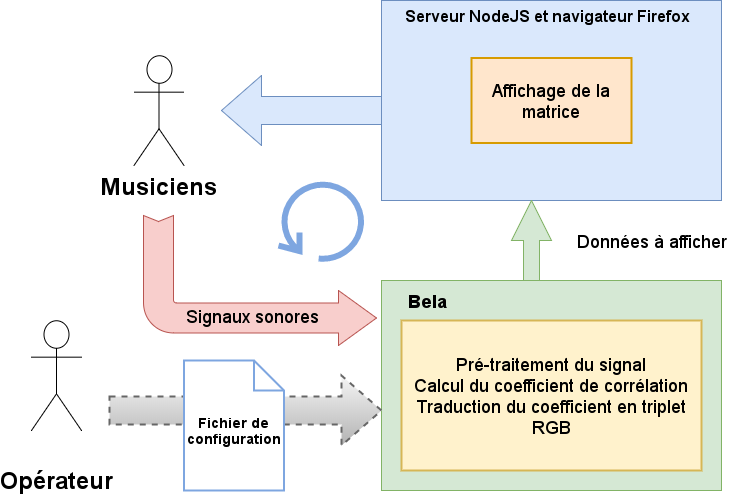
\includegraphics[scale=0.5]{assets/VisualImpro.png}
 \caption{Schéma global du dispositif de VisualImpro}
 \label{schéma global}
\end{figure}

\paragraph{}
Ci-dessus, un schéma global du fonctionnement du dispositif. Les
musiciens jouent un morceau traité par Bela qui, via l'intermédiaire
d'une machine, affiche sur le navigateur web Mozilla Firefox la
matrice graphique de corrélations censée assister le jeu des
musiciens.

\paragraph{}
Différentes pistes ont été proposées par Jérémy dans son rapport pour
améliorer le logiciel produit : implémenter un retour sonore indiquant
aux musiciens la qualité des corrélations en fonction du coefficient
calculé à la place du retour visuel, ajouter des effets audio aux
pistes sonores en amont du calcul de corrélation...
